\documentclass{article}      % Specifies the document class

\usepackage{amsmath}
\usepackage{algpseudocode}
\usepackage{algorithm}
\usepackage{forloop}
\usepackage{graphicx}

\usepackage{subcaption}


\newcounter{ct}
\newcommand{\markdent}[1]{\forloop{ct}{0}{\value{ct} < #1}{\hspace{\algorithmicindent}}}
\newcommand{\markcomment}[1]{\Statex\markdent{#1}}

\algnewcommand\algorithmicforeach{\textbf{for each}}
\algdef{S}[FOR]{ForEach}[1]{\algorithmicforeach\ #1\ \algorithmicdo}

\begin{document}
 \large Intro about re project \\
 \large BDD Modeling Process \\


     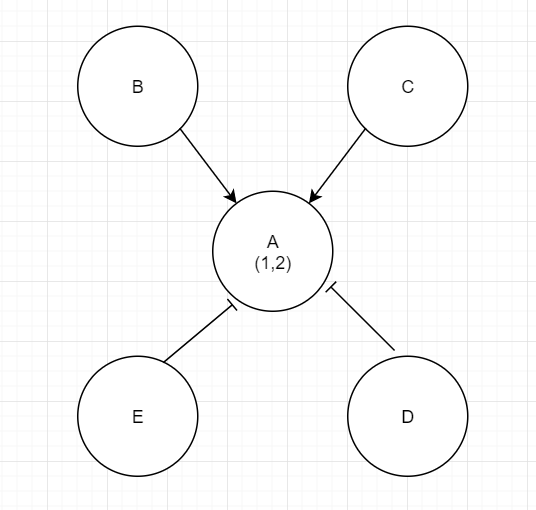
\includegraphics[width=3cm, height=3cm]{ex1.png}
We can see node A have two positives activators (B, C) and two repressors (D,E). The number inside A mark that A next value is set by two possible functions, function 1 and function 2. In this case function number 1 is “OrNegativeIsTrue” that mean one of all the repressors is activated and Function number 2 is “AndPositiveIsTrue” that mean all activators are needed to be on. 
Because Node A is controlled by one of this two functions, so we need to put an OR operator between them.
The observation for this example is:
\begin{table}[h]
\begin{tabular}{|l|l|l|l|l|l|}
\hline
\textbf{Time} & \textbf{A} & \textbf{B} & \textbf{C} & \textbf{D} & \textbf{E} \\ \hline
0             &            & 0          & 1          & 1          & 1          \\ \hline
1             & 1          &            &            &            &            \\ \hline
\end{tabular}
\end{table}
Now we have to decide if one of the function of node A can satisfy the observation we take. To perform this, we digital every function with following notation:
#F2\_A , mean function number 2 is selected function to node A.
We have to ensure that one (but more than one is right too) of the function will be selected, so we add an “or” function between the two functions.
To do that we have to calculate the function of A for every t.
\[  a_1 = 1 \wedge b_0 = 0 \wedge c_0 = 1 \wedge d_0 = 1 \wedge e_0 = 1 \wedge

\\
(#F_1_a \vee #F_2_A) \wedge
\\
((#F_1_a \wedge (e_0 \vee d_0))) \vee 
\\
(#F_2_a \wedge (b_0 \wedge c_0))
 \]

The BDD that will be created for this expression is:
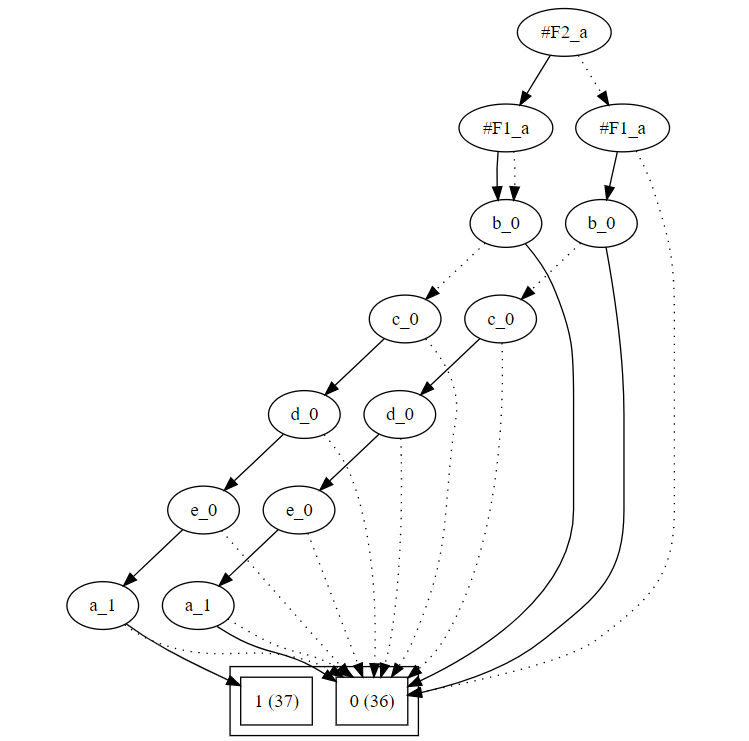
\includegraphics[width=6cm, height=8cm]{bdd1.png}
From the BDD we can extract needed information. The equation have a single solution (only one arrow arrive to “1” box, and Function 2 must be choose to have a valid solution.



\large Optional Connections \\
Another problem we had to deal in “re” modeling is the existence of optional connections. In the network model we have some connections that we are sure they exist, but we have other connections that can be enabled or disabled. The goal of “re” project was to determine which of these connections are enabled and which are disabled. In biologic world a connection means a gene have an influence on another gene. In our BDD modeling we had to find a way to digitalize this optional connections. In next figure we have the same Boolean network as in last example, but in this example connection between B and A is optional.
To deal with this feature we add another bit that signal if the connection exists or nope. In our example, we will add a parameter called R\_A\_B (relation between A and B). We have to update the equation to support optional connections feature.
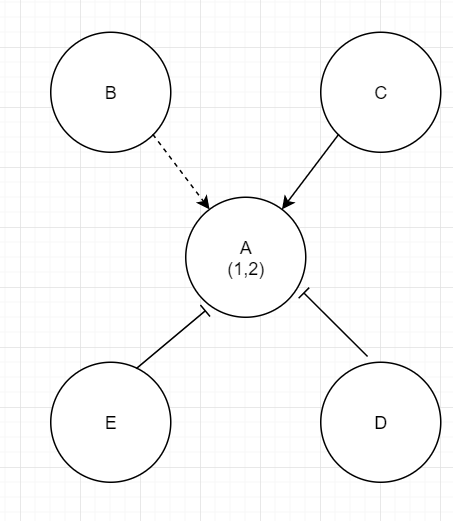
\includegraphics[width=6cm, height=8cm]{image11.png}

Updated equation is like this:
\[
a_1 = 1 \wedge b_0 = 0 \wedge c_0 = 1 \wedge d_0 = 1 \wedge e_0 = 1 \wedge
\\

(#F_1_a \vee #F_2_A) \wedge
\\

((#F_1_a \wedge (e_0 \vee d_0))) \vee 
\\

(#F_2_a \wedge ((\overline{R_A_B} \vee b_0) \wedge c_0))
\]

The logic we found to fulfill this feature is that in every OR function the optional parameter is involved we will add an AND function with the new bit.

For example:
\[
\\
a_1 = b_0 \wedge c_0
\]

will become:
\[
a_1 = (R_A_B \wedge b_0) \vee c_0
\]

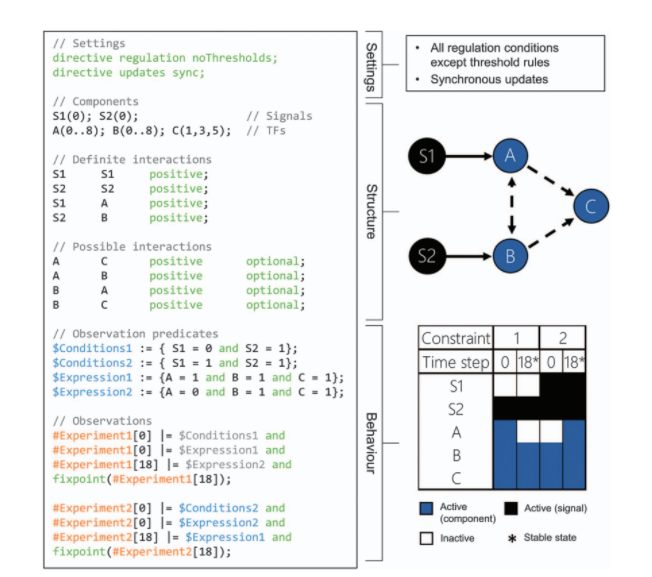
\includegraphics[width=6cm, height=8cm]{image14.png}
Figure – We can see that in experiment1 we have results only for time slots 0 and 18. In experiment number 1 and time slot 18 we have predicates called \$expression2 that have values only for A,B and C, we don’t have values at this timeslot for S1 and S2.

\begin{table}
    \begin{tabular}{llllll}
    ~  & s1 & s2 & A & B & C \\
    0  & 0  & 1  & 1 & 1 & 1 \\
    18 & ~  & ~  & 0 & 1 & 1 \\
    \end{tabular}
\end{table}


In real examples, we can have more than 10 different experiments in the same observation files. The pattern matching process is to find which functions and which optional connection are used to fulfill the different experiments. In sometimes we found contradiction between observation results and networks, it can signal the observation are not accurate. 
Processing high amount of observations with SMT or BDD solvers can be a hard job even for high performance machine.
Our solution suggests adding a pre-process step that can merge and union one or multiple observation results to a smaller set. To perform this step, we try to merge two experiments and check if there is not any contradiction in condition results, and check too the new experiment result fulfill network conditions. This process run iteratively with a backtracking mechanism until we can’t merge together more experiments. An already merged experiment can be merged again with other experiment if not any contradiction will be found. Because we try to merge two experiments results in multiple time-slots, the result of merges between two experiments is not a single merged, but can be a set of multiple merges candidates. To distinguish every different merge, we mark the new merge with a “~” sign, and add the two involved experiments. Because the merge can be created from two different timeslots in every experiment, we add the timeslots too. For example, from Exp1 and Exp2, we can have a merge with label “Exp1\_10 \~ Exp2\_14”, meaning experiment 1 in timeslot 10 is merged with experiment2 in timeslot 14.
A merge from two experiments don’t have to be in same timeslot from the two experiments, because the time in the experiments is not absolute time, but relative time for this specific experiment. Although we assume the all timeslots are from the same length, the experiments don’t have to be with the same length, in some case one experiment will be “shallowed” in second experiment, and in some case the tail of an experiment will continue after merged part. A special case is when that last timeslot of an experiment can be merged to the first timeslot of the second experiment. In this case we will have one long experiment with the value of the first one, and after that the values of the second one.

\large Loop \\
Another improvement we propose in “re” modeling, is the existence of loops in experiments. Experiments results we have are sometime very long (more than 20 steps), but there are also with a very low density of data.  That mean Pattern Matching process is very long and need a lot of computation power. In some cases the experiment arrive to “Dead end”. In some experiments from a time slot the results are constants. In “re” process they pass over all the slots. Our algorithm can identify this “Dead end” or “loop” states and recreate a new experiment that will be less long. That will make all the process faster.


\pagebreak

\begin{algorithm} \caption{Process Experiments List}
\begin{algorithmic}[1]
\Function {ProcessExperiments}{}
\State $list \gets \text{list of experiments}$
\State $booleanNetwork \gets \text{boolean network graph and functions}$
\State \textbf{begin function}
    \ForEach {$e_1$, $e_2$ pair of experiments in list}
        \State $res \gets FindValidMerges(e_1, e_2, bn)$
        \If{\text{res has values}}
                \State $newList \gets \text{a copy of experiments list}$
        \State \text{add res to top of the list (can be multiple)}
        \State \text{call} $ProcessExperiments(newList, booleanNetwork)$
        \EndIf
        
        
    \EndFor
        \If{\text{not any valid merge in list }}
                \State{Add list to ReusltList}
        \EndIf
\EndFunction

\end{algorithmic}
\end{algorithm}
\begin{algorithm}
\begin{algorithmic}[1]
\Function {FindValidMerges}{}
\State $exp1 \gets \text{first experiment}$
\State $exp2 \gets \text{second experiment}$
\State $booleanNetwork \gets \text{boolean network graph and functions}$
\State \textbf{begin function}
    \ForEach {s state in exp1}
        \State $mergedExperiment \gets \text{connect s with begin of exp2}$
        \If{\text{IsValidMerge(mergedExperiment, booleanNetwork)}}
                \State \text{add mergedExperiment to returnList }
        \EndIf
    \EndFor
    \ForEach {s state in exp2}
        \State $mergedExperiment \gets \text{connect s with begin of exp1}$
        \If{IsValidMerge(mergedExperiment, booleanNetwork)}
                \State \text{add mergedExperiment to returnList }
        \EndIf
    \EndFor
\EndFunction
\end{algorithmic}
\end{algorithm}
\begin{algorithm}
\begin{algorithmic}[1]
\Function {IsValidMerge}{}
\State $exp \gets \text{an experiment}$
\State $booleanNetwork \gets \text{boolean network graph and functions}$
\State $bdd \gets \text{an new empty BDD}$
\State \text{Add states values to BDD}
\State $BDD \gets \text{an empty BDD}$
\State \textbf{begin function}
    \ForEach {\text{s state in experiment}}
        \State $BDD \gets \text {BDD $\vee$ s}$
    \EndFor
\State $functionBDD \gets \text{an empty BDD}$
    \ForEach {\text{v vertex in booleanNetwork}}
        \State $incomeEdges \gets \text{income edges to vertex v}$
        \State $availableFunctions \gets \text{available functions for vertex v}$
        \State $functionBDD \gets \text{functionBDD AND CreateFunctionRepresentation(v, availableFunctions, incomeEdges, experiment.length)}$
    \EndFor
\State $BDD \gets \text{BDD AND functionBDD}$
\State $BDD \gets \text{BDD AND 1}$
\If{BDD is Empty}
    \State \text{return false}
\EndIf
    \State \text{return true}
\EndFunction
\end{algorithmic}
\end{algorithm}
\begin{algorithm}
\begin{algorithmic}[1]
\Function {CreateFunctionRepresentation}{}
\State $availableFunctions \gets \text{list of possible functions}$
\State $letter \gets \text{current letter}$
\State $edges \gets \text{list of edges letter}$
\State $length \gets \text{experiment length}$
\State \textbf{begin function}
\State $functionBDD \gets \text{an empty BDD}$
    \For{\texttt{i=0;i<length;i++}}
        \State $tempBDD \gets \text{an empty BDD}$
        \ForEach {\text{F function in availableFunctions}}
            \State $tempBDD \gets \text{tempBDD OR ($f_i$ and $F_i$implementation(edges))}$
            \State \Comment{Missing part: optional parameters}
        \EndFor
        \State $tempBDD \gets \text{tempBDD AND (f1, f2, .., fn}$
        \State \Comment{ensure one of the function has been choosen}
        \State $functionBDD \gets \text{functionBDD AND $letter_{i+1}$ equal tempBDD}$
    \EndFor
    \State \text{return functionBDD}
\EndFunction
\end{algorithmic}
\end{algorithm}

\end{document}